\chapter{Introduction}\label{cha:intro}
\epigraph{``In mesoscopic physics, you really need to build up intuition, because it is not the world you know.''}{Carlo Beenakker~\cite{beenaker_quote}}



\section{Context}

\begin{figure}[!htb]
 \begin{center}
%% psfrag: comment the following line if not using the psfrag package
 % \psfrag{pie makes me happy!}{$\pi$ makes me happy!}
%% includegraphics: comment the following if not using the graphicx package
 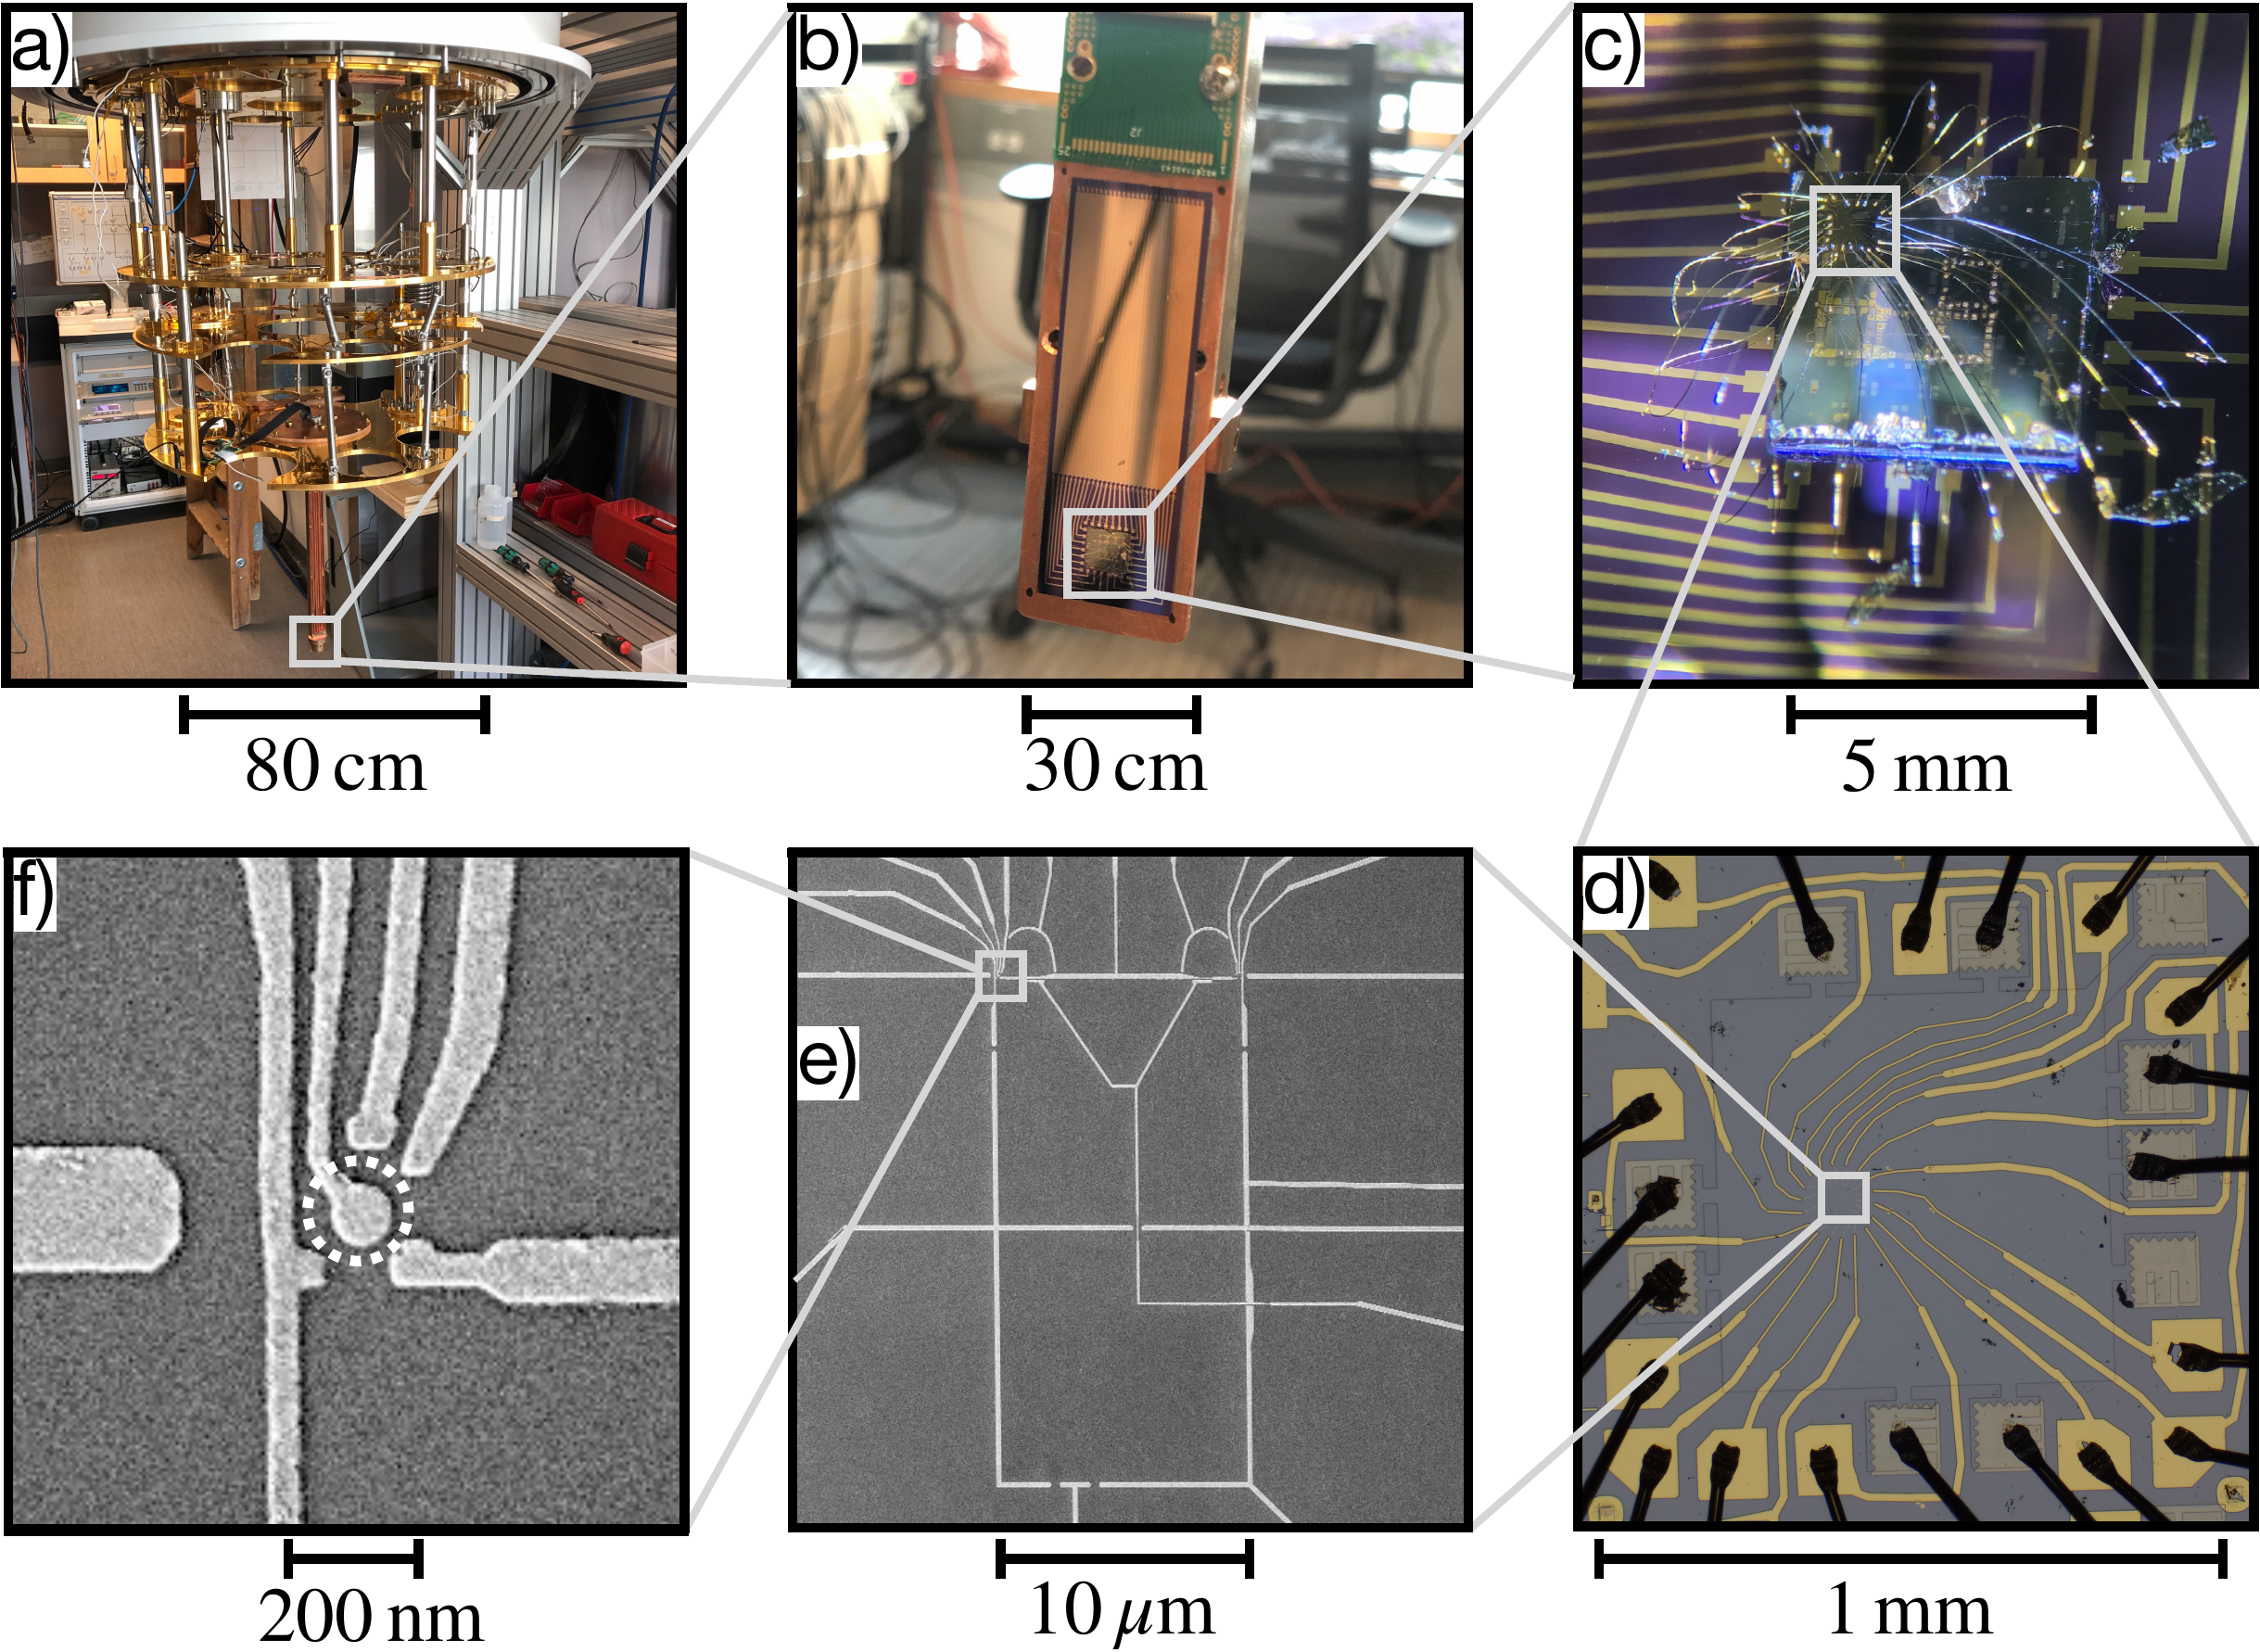
\includegraphics[width=0.95\textwidth]{figures/ch1/figure1.pdf}
 \caption[Fridge to Quantum Dot Scale Illustration]{\label{fig:ch1/scale_breakdown} 
 % For some options that work with pdf\LaTeX, please see this discussion:
 % \url{http://tex.stackexchange.com/questions/11839}. 
Illustrating the relationships from macroscopic to nanoscale to demonstrate the tunability of quantum devices. (\textbf{a}) Photograph of the Au-plated cold plates within a dilution refrigerator. The lowest plate, known as the mixing chamber, can reach temperatures of \qty{8}{mK}. (\textbf{b}) Photograph of the Si chip carrier, onto which the heterostructure is stuck. (\textbf{c}) An optical microscope image shows the heterostructure attached to the chip carrier. Thin Al wire bonds connect the quantum device to the fridge wires. (\textbf{d}) Optical microscope image of a single mesa on the heterostructure. A mesa is an isolated area of the heterostructure where new designs are fabricated. The black lines around the outside are wire bonds and the bright Au are thick (\qty{100}{nm}) `outer gates' which connect to thin (\qty{10}{nm}) `inner gates'. (\textbf{e}) Scanning electron micrograph (SEM) of the inner gates. The mean free path of the electrons is of order \qty{3}{\mu m}. (\textbf{f}) SEM image of the quantum dot. An isolated puddle of electrons with a total occupation of 0 - 10 is engineered by carefully tuning the voltages on the inner gates. 
  }
 \end{center}
\end{figure}




\noindent Mesoscopic physics is in the domain of condensed matter physics with system scale sizes between nanometer and micrometre. Mesoscopic systems unveil a rich zoo of quantum phenomena and material properties. 
Distinct from their macroscopic counterparts, mesoscopic systems can exhibit behaviour influenced by quantum effects. One of the initial measurements of a mesoscopic system studied the conductance through a quantum wire~\cite{qpc_first_measurement, qpc_second_measurement}. 
Classically, the conductance is expected to be proportional to the width of the wire. 
However, as the width varies, it was found that a quantum wire exhibits steps at integer conductance values. Each step in conductance 
is the result of an additional 1d-suband that contributes to the transport. Another milestone in the field was the discovery of Coulomb blockade oscillations in the conductance measured across a quantum dot~\cite{first_charging_of_qd}. 
In this experiment, a small isolated island of electrons was connected to two baths of electrons through tunnel barriers. 
The island's small size results in charge quantisation and significant spacing between orbital energy levels, forming an `artificial atom'. 
The benefits of this system come from a high degree of tunability and control. The relevant scales that allow human control over this `artificial atom' are illustrated in Fig.~\ref{fig:ch1/scale_breakdown}.
The scope of mesoscopic physics is continually expanding, with ongoing developments in new materials~\cite{manfra_inas}, measurement methods~\cite{child_meas}, and arrangement of systems~\cite{borsoi2022shared, raysu}.

Theorists and experimentalists enjoy a symbiotic relationship in mesoscopic physics. Experiments validate established theories, while theorists are tasked with modelling surprising and repeatable phenomena discovered in experiments. Notable examples of successful experiments validating theory include the investigation of Wigner crystals~\cite{wigner_solid}, isolation of graphene~\cite{graphene}, and measurement of the charge of quasiparticles in the fractional quantum Hall effect~\cite{fractional_charge}. Conversely, instances of unexpected experimental findings that prompted theoretical inquiry include integer quantum Hall effect~\cite{klitzing}, anomalous Landau quantisation~\cite{landau_quantisation}, and superconductivity in twisted double bilayer graphene~\cite{raysu}.

This thesis focuses on a phenomenon initially discovered through experimental observation, prompting theorists to develop a new model capable of predicting the striking behaviour observed in measurements. The `Kondo effect', first discovered in impure bulk metals in the 1930s~\cite{de_haas} and explained later in the 1960s~\cite{jun_kondo}, has seen significant interest in the field of quantum devices. These devices offer high tunability and control, allowing for testing theoretical predictions~\cite{costi_kondo_mv_eo_regime}. 
The Kondo effect in quantum devices involves a net spin (odd number of electrons) in a quantum dot that is strongly coupled to two electron reservoirs (leads). Virtual tunnel events through the quantum dot, with possible spin flips, lead to a correlated state called the Kondo singlet. The Kondo effect can be seen in the enhanced conductance between Coulomb peaks with decreasing temperature. This conductance approaches the unitary limit, where the transmission probability through the quantum dot is one~\cite{kondo_unitary, kondo_unitary_theory, yigal_kondo}. This is a remarkable effect as the tunnel barriers into the quantum dot each have a transmission probability less than one. More recent experiments have explored exotic regimes of the Kondo effect. For example, Kondo effect in graphene~\cite{kondo_graphene}, Kondo lattices which are used to study quantum criticality~\cite{kondolattice}, multi-channel Kondo which could lead to non-Fermi liquid
behaviour~\cite{potok_2ck, iftikhar_2ck, kirchner_2ck}, and the novel topological Kondo effect which could demonstrate the non-local quantum dynamics of Majorana fermions~\cite{topological_kondo_majorana, topological_kondo, kondo_topological}.

Nevertheless, there remains considerable potential for further insights by extending the scope of the initial, seemingly 'simple' measurements on the Kondo effect into new parameter regimes. In this thesis, we develop and test a novel method for measuring the Kondo effect with weaker coupling than previously explored. This regime is rarely explored as the conductance enhancement from Kondo is small, and cannot be reliably with a conductance measurement only. Interestingly, a recent measurement of entropy in this regime found a disagreement with theoretical predictions~\cite{child_strong}. Hence, this measurement of conductance taken in a similar regime could illuminate the reasons for the discrepancy.




\section{Outline}


Chapter~\ref{cha:device_background} provides an overview of quantum devices. The chip material (GaAas/AlGaAs heterostructure) is introduced and how metal gates on top of the chip are used to engineer quantum structures such as quantum point contacts and quantum dots. Also, measurements of conductance and occupation through a quantum dot are described.


Chapter~\ref{cha:kondo_conductance} introduces the Kondo effect in bulk materials and quantum dots. It includes a measurement demonstrating the large conductance enhancement caused by the Kondo effect in the `Kondo regime', highlighting the differences from the regime discussed in the subsequent Chapter~\ref{cha:mixed_valence_conductance}.



Chapter~\ref{cha:mixed_valence_conductance} demonstrates a method to measure the conductance enhancement from the Kondo effect with weaker coupling. Various dot configurations are tested, with results compared to the Numerical Renormalization Group (NRG) theory.



Chapter~\ref{cha:conclusion} consolidates the main findings from Chapter~\ref{cha:mixed_valence_conductance}, and outlines future directions for this research.